\documentclass[answers]{exam}

\usepackage{amsmath}
\usepackage[spanish]{babel}
\usepackage[T1]{fontenc}
\usepackage{graphicx}
\usepackage{lmodern}
\usepackage{wrapfig}

\extrawidth{1.04cm}
\extraheadheight[3cm]{-5mm}
\extrafootheight[-5mm]{-2mm}
\renewcommand{\familydefault}{\sfdefault}
\graphicspath{{../../Imagenes/}{Imagenes/}}

\newcommand{\materia}{Organización y \\ Arquitectura de Computadoras}
\newcommand{\tarea}{Tarea 4}
\newcommand{\titulo}{Circuitos Digitales}
\newcommand{\fecha}{28 de Octubre de 2021}

\firstpageheader{
  \setlength{\intextsep}{2.2em}
  \begin{wrapfigure}{l}{3.7cm}
    \centering
    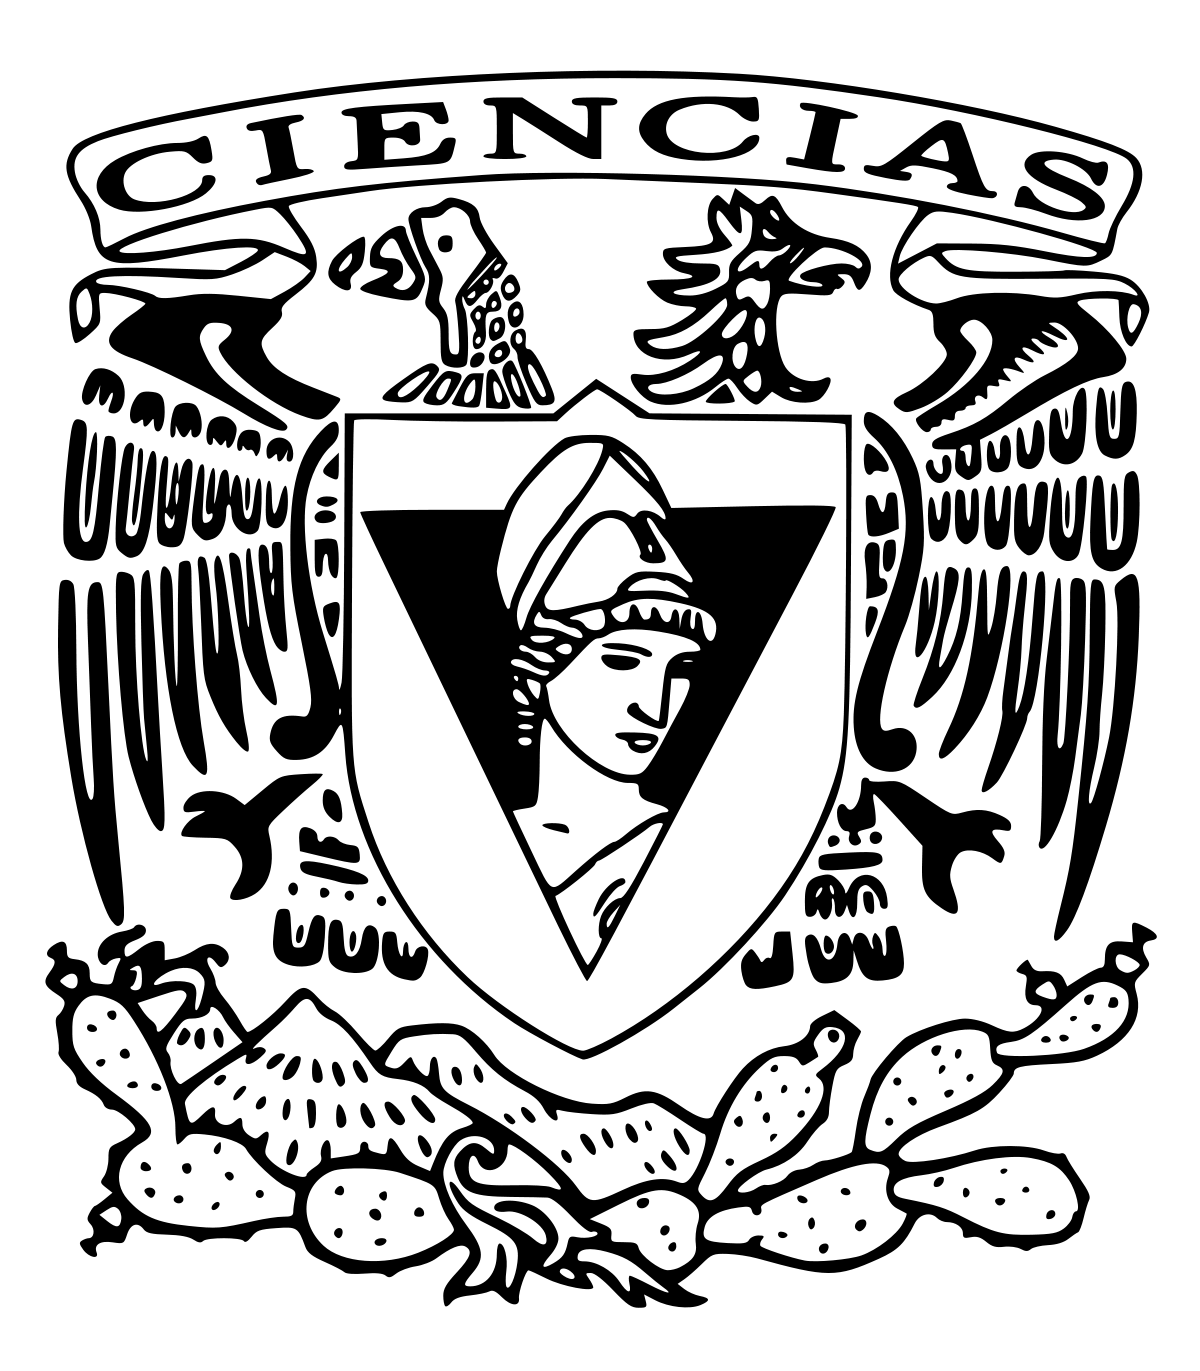
\includegraphics[scale=0.09]{fc}
  \end{wrapfigure}
  \hfill\break{} \\[3.5mm]
  \LARGE\textbf{\materia} \\
  \LARGE\textbf{\tarea: \titulo} \\[4pt]
  \large\textbf{Facultad de Ciencias, UNAM} \\[4pt]
  \textbf{José Ethan Ortega González:} 316088327 \\
  \textbf{Etzael Iván Sosa Hedding:} 316259305 \\
}{}{
  \setlength{\intextsep}{-12.5em}
  \begin{wrapfigure}{l}{3.3cm}
    \centering
    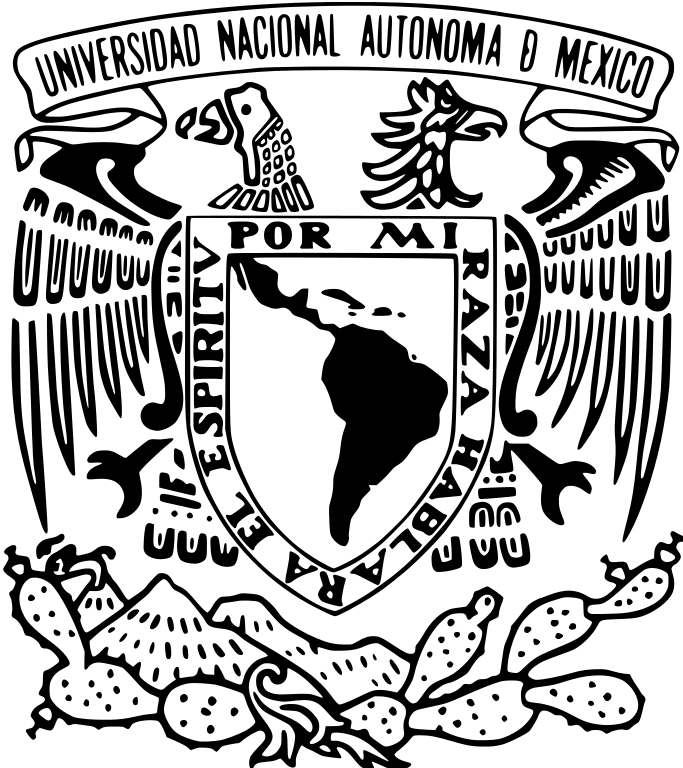
\includegraphics[scale=0.15]{unam}
  \end{wrapfigure}
}

\renewcommand{\solutiontitle}{\noindent\textbf{Solución:}\par\noindent}
\renewcommand{\thequestion}{\textbf{\arabic{question}}}
\runningheadrule{}
\runningfootrule{}
\firstpagefootrule{}
\runningheader{\materia}{\tarea}{\fecha}
\footer{}{Página \thepage\ de \numpages}{}

\begin{document}
\begin{questions}
  \question{De las siguientes funciones dibuje los diagramas lógicos
    correspondientes.}
  \begin{itemize}
    \item $\neg(p \land q) \leftrightarrow \neg p \lor \neg q$
    \item $p \lor (p \land q) \leftrightarrow p$
    \item $p \land q \lor r \to q$
    \item $((p \to q) \land (q \to r)) \to (p \to r)$
  \end{itemize}

  \question{Dibuje los diagramas lógicos para AND, OR y NOT usando compuertas
    NAND.}

  \question{En base a diagramas de transistores NMOS tipo NPN, represente el
    siguiente circuito.}
  \begin{center}
    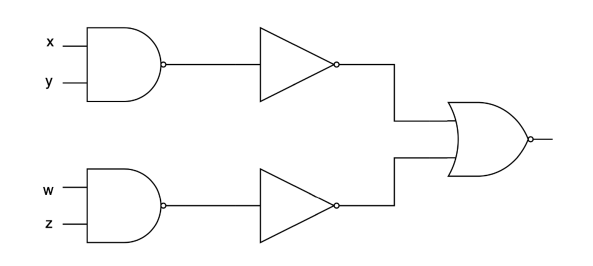
\includegraphics[scale=0.5]{circuito}
  \end{center}

  \question{En base al circuito anterior, da su tabla de verdad asociada. ¿Puede
    este circuito utilizarse como una compuerta NAND y también como una
    compuerta NOR?\@ En caso de ser afirmativa la respuesta, justifíquela.}
  \begin{solution}
    No puede ser utilizada como una compuerta NOR, solo puede ser utilizada como
    una compuerta NAND.\@ Sea $F$ la salida del circuito del ejercicio, la tabla
    de verdad del circuito y del NAND de $4$ bits:
    \begin{gather*}
      \begin{array}{c|c|c|c|c|c}
        x & y & w & z & F & NAND \\
        \hline
        0 & 0 & 0 & 0 & 1 & 1 \\
        0 & 0 & 0 & 1 & 1 & 1 \\
        0 & 0 & 1 & 0 & 1 & 1 \\
        0 & 0 & 1 & 1 & 1 & 1 \\
        0 & 1 & 0 & 0 & 1 & 1 \\
        0 & 1 & 0 & 1 & 1 & 1 \\
        0 & 1 & 1 & 0 & 1 & 1 \\
        0 & 1 & 1 & 1 & 1 & 1 \\
        1 & 0 & 0 & 0 & 1 & 1 \\
        1 & 0 & 0 & 1 & 1 & 1 \\
        1 & 0 & 1 & 0 & 1 & 1 \\
        1 & 0 & 1 & 1 & 1 & 1 \\
        1 & 1 & 0 & 0 & 1 & 1 \\
        1 & 1 & 0 & 1 & 1 & 1 \\
        1 & 1 & 1 & 0 & 1 & 1 \\
        1 & 1 & 1 & 1 & 0 & 0 \\
      \end{array}
    \end{gather*}
  \end{solution}

  \question{Dibuje los diagramas lógicos de las siguientes funciones. En caso de
    que la función no sea óptima, utilice el método a conveniencia visto en la
    tarea anterior para reducirla.}
  \begin{itemize}
    \item
          \begin{math}
            F(x_{0}, x_{1}, x_{2}) = x_{0}x_{1}x_{2} + \overline{x_{0}x_{1}x_{2}} +%
            x_{0}x_{1}\overline{x_{2}} + \overline{x_{0}x_{1}}x_{2}%
          \end{math}
    \item
          \begin{math}
            F(x_{0}, x_{1}, x_{2}, x_{3}) = \overline{x_{0}x_{1}x_{2}x_{3}} +%
            \overline{x_{0}x_{1}x_{2}}x_{3} + \overline{x_{0}x_{1}}x_{2}x_{3} +%
            x_{0}x_{1}\overline{x_{2}x_{3}} + x_{0}x_{1}x_{2}\overline{x_{3}}
          \end{math}
    \item
          \begin{math}
            \begin{aligned}[t]
              F(x_{0}, x_{1}, x_{2}, x_{3}, x_{4}) =\;
              &\overline{x_{0}x_{1}x_{2}x_{3}x_{4}} +
              \overline{x_{0}x_{1}}x_{2}x_{3}\overline{x_{4}} +
              x_{0}\overline{x_{1}}x_{2}x_{3}x_{4} \\
              &+ x_{0}x_{1}\overline{x_{2}x_{3}}x_{4}
              + \overline{x_{0}}x_{1}\overline{x_{2}x_{3}}x_{4}
              + x_{0}x_{2}x_{3}x_{4}
            \end{aligned}
          \end{math}
  \end{itemize}

  \question{Dibuje el diagrama lógico de un sumador completo de 4 bits.}

  \question{Utilizando sumadores y semi-sumadores, diseña un circuito digital
    que realice resta entre numero de 8 bits.}

  \question{Utilizando sumadores y semi-sumadores, diseña un circuito digital
    que realice multiplicación entre numero de 4 bits.}

  \question{Minimizando la cantidad de sumadores completos ¿Cómo quedaría la
    suma entre dos números de 32 bits? ¿Cuántos sumadores completos se
    requerirían?}

  \question{Diseña un circuito digital que resuelva la siguiente ecuación:
    $x = 2y + z$}
\end{questions}
\end{document}
